% Provenance (never printed): old terminale S material on the transformation of
% rocks in mountain belts and subduction zones (pressure, temperature, index
% minerals and the Al2SiO5 polymorphs, foliation, contact and regional
% metamorphism). Owner (Sync 0): metamorphism, lithostatic pressure, polymorph,
% index mineral/isograd/metamorphic grade, foliation/schistosity, contact and
% regional metamorphism/aureole. Blueschist and eclogite are g11.06's, the
% geotherm g11.03's, minerals and silicates g11.07's, the rock families, marble
% and slate Book 1's (g6), pressure physics': recalled, never redefined. The
% P-T diagram: figdata/grade-12/al2sio5.py (Holdaway and Mukhopadhyay 1993,
% Table 11; geotherms from Earle 7.3).
\chapter{الصخور المتحولة}\label{ch:g12:metamorphic-rocks}

تستقر طبقة من الوحل على قاع بحر وتتصلب فتصير سجيلًا. ادفنها بضعة
كيلومترات واعصرها، فتصير أردوازًا، وهو صخر ينشق إلى
الصفائح الرقيقة المستوية التي تُسقف بها البيوت. وادفنها أعمق وأسخن، فتنمو رقائقها الدقيقة
إلى ميكا لامعة، تنتفخ بينها حبات العقيق الحمراء: إنه الشيست.
وأعمق وأسخن من ذلك أيضًا، تتمايز معادنها في أشرطة فاتحة وداكنة:
إنه النيس. ولم ينصهر شيء على طول الطريق. فالوحل نفسه، بالعناصر
الكيميائية نفسها، أعاد ببساطة بناء معادنه لتلائم المكان الذي
كان فيه. وإذا قُرئ الأمر في الاتجاه المعاكس، فإن معادن الصخر المتحول تسجّل مدى عمق
ذلك المكان ومدى سخونته، وهذا الفصل يتعلم قراءتها.
% ledger: earle:foliation, earle:settings

\begin{recall}
تنقسم الصخور ثلاث عائلات --- نارية، ورسوبية، ومتحولة ---
ودورة الصخور تحوّل إحداها إلى أخرى؛ فالرخام يُصنع من الحجر الجيري
والأردواز من السجيل، دون انصهار (الكتاب 1، الصف 6). والمعدن مادة صلبة
طبيعية لها تركيب كيميائي محدد وترتيب منتظم
للذرات؛ ومعظم معادن القشرة \omterm{def:g11:minerals:silicate}{سيليكات}
(\cref{ch:g11:minerals}). \omterm{def:g11:lithosphere-asthenosphere:geotherm}{والمنحنى الحراري الأرضي} هو منحنى درجة الحرارة بدلالة
العمق تحت مكان ما؛ وقرب السطح ترتفع درجة الحرارة بمقدار 25 إلى
\qty{30}{\celsius} لكل كيلومتر (\cref{ch:g11:lithosphere-asthenosphere}).
وفي \omterm{def:g11:subduction-zones:subduction}{نطاق الاندساس}، تتحول \omterm{def:g11:ocean-ridges:oceanic-lithosphere}{القشرة المحيطية} التي تُحمل إلى الأسفل وهي باقية باردة
إلى \omterm{def:g11:subduction-zones:eclogite}{شيست أزرق}، ثم إلى \omterm{def:g11:subduction-zones:eclogite}{إكلوجيت} (\cref{ch:g11:subduction-zones}).
والضغط قوة مقسومة على المساحة التي تضغط عليها؛ ويُقاس
بالباسكال، \qty{1}{Pa} = \qty{1}{N/m^2}.
\end{recall}
% ledger: usgs:metamorphic (Book 1 row), webmineral:formulas, earle:settings, earle:controls

\section{تحول في الحالة الصلبة}

\begin{definition}[التحول]\label{def:g12:metamorphic-rocks:metamorphism}
\emph{التحول}\index{تحول (الصخور)} هو تغير
معادن الصخر \omterm{def:g11:igneous-rocks:texture}{ونسيجه}، في الحالة الصلبة، حين يُنقل
إلى درجة حرارة وضغط مختلفين عن اللذين تكوّن فيهما.
والصخر الذي يصير إليه صخر متحول.
\end{definition}
% ledger: tulane:metamorphism, earle:controls

الصخر الذي يبدأ منه \omterm{def:g12:metamorphic-rocks:metamorphism}{التحول} هو صخره الأم، وهي العبارة نفسها
المستعملة للصخر الذي تحت التربة (\cref{ch:g10:soil-formation}). ويبدأ \omterm{def:g12:metamorphic-rocks:metamorphism}{التحول} عند نحو \qty{200}{\celsius}؛ وتحت ذلك، تنتمي التغيرات
البطيئة للراسب المدفون إلى تصلبه وصيرورته صخرًا. وينتهي
حيث يبدأ الصخر بالانصهار: ومنذئذ يكون ما يحدث ناريًا. وبين
هذين الحدين، لا يكون كل معدن مستقرًا إلا في مدى معين من
درجة الحرارة والضغط. فمعظم \omterm{def:g10:soil-formation:clay}{المعادن الطينية}، مثلًا، لا تدوم إلا حتى
نحو 150 أو \qty{200}{\celsius}؛ وفوق ذلك تتحول إلى ميكا. وحين
تتغير الظروف، تعيد ذرات المعادن غير المستقرة ترتيب نفسها،
حبةً حبةً، في معادن مستقرة في الظروف الجديدة.
% ledger: tulane:metamorphism, earle:controls

أربعة أمور تتحكم في النتيجة. \textbf{\omterm{def:g10:soil-formation:weathering-profile}{الصخر الأم}} يوفّر
العناصر الكيميائية: فالحجر الجيري المكوّن من الكالسيت وحده لا يصير إلا
رخامًا مكوّنًا من الكالسيت. و\textbf{درجة الحرارة} و\textbf{الضغط} يحددان أي
المعادن مستقرة. و\textbf{الماء}، الموجود بكميات صغيرة بين
الحبيبات، ينقل الأيونات الذائبة من حبة إلى أخرى ويسرّع
التفاعلات. \omterm{def:g12:metamorphic-rocks:metamorphism}{والتحول} بطيء: فالمعادن الجديدة تنمو بنحو مليمتر
في مليون سنة. والأحداث التكتونية التي تدفن الصخور بطيئة أيضًا، فيكون
للتفاعلات عادةً متسع من الوقت لتكتمل.
% ledger: earle:controls

\subsection{وزن الصخور التي فوقه}

الصخر المدفون على عمق $z$ يحمل وزن كل الصخور التي فوقه.

\begin{definition}[الضغط الصخري]\label{def:g12:metamorphic-rocks:lithostatic}
\emph{الضغط الصخري}\index{ضغط صخري} عند عمق $z$
هو الضغط الذي يؤثر به على الصخر وزنُ عمود الصخور الذي
فوقه. وهو متساوٍ في كل الاتجاهات.
\end{definition}
% ledger: earle:controls (confining pressure, equal in all directions), tulane:metamorphism

\begin{proposition}[الضغط الصخري]\label{prop:g12:metamorphic-rocks:lithostatic}
تحت عمود من الصخر كثافته منتظمة $\rho$، يكون \omterm{def:g12:metamorphic-rocks:lithostatic}{الضغط الصخري}
عند العمق $z$
\[
  P = \rho g z ,
\]
حيث $g$ تسارع الجاذبية؛ ويُهمَل ضغط
الغلاف الجوي، نحو \qty{0.1}{MPa}.
\end{proposition}

\begin{proof}
خذ عمودًا رأسيًا من الصخر مقطعه الأفقي $A$، من
السطح نزولًا إلى العمق $z$. حجمه $Az$، وكتلته $\rho A z$،
ووزنه $\rho A z g$. وهذا الوزن يستقر على المساحة $A$ في أسفل
العمود، فيكون الضغط هناك $P = \rho A z g / A = \rho g z$.
\end{proof}

مع متوسط كثافة \omterm{def:g12:continental-crust:continental-crust}{القشرة القارية}، $\rho = \qty{2830}{kg/m^3}$،
و$g = \qty{9.81}{m/s^2}$، يرتفع الضغط بمقدار $\rho g = 2830 \times 9.81
\approx \qty{27800}{Pa}$ لكل متر، أي نحو \qty{27.8}{MPa} لكل
كيلومتر. وعند قاعدة قشرة سمكها \qty{35}{km} يبلغ
\[
  P = 2830 \times 9.81 \times \num{35000} \approx \qty{9.7e8}{Pa} \approx
  \qty{0.97}{GPa},
\]
أي نحو \qty{1}{GPa}: ما يقارب عشرة آلاف ضعف ضغط الغلاف الجوي
عند مستوى سطح البحر. وكثيرًا ما تُقرأ الضغوط في الاتجاه المعاكس، أعماقًا:
فالضغط \qty{1}{GPa} يُبلغ على عمق $\num{e9}/(2830 \times 9.81) \approx \qty{36}{km}$
تحت السطح.
% values: P_35km_gpa 0.97168, dPdz_mpa_per_km 27.762, z_1gpa_km 36.02 (al2sio5.py)
% ledger: cm95:crust; Book 1: ussa76:sea-level (101 325 Pa, g0 = 9.80665 m/s2)

وزن الصخور يضغط بالتساوي من كل الجهات. وفي الحزام الجبلي،
تضيف الصفائح دفعًا في اتجاه واحد: فيُعصر الصخر من
الجانبين بشدة أكبر منها من الأعلى. وهذا الضغط \emph{الموجَّه} لا يغيّر أي
المعادن مستقرة، لكنه يغيّر كيفية ترتيبها، كما
يُظهر \cref{sec:g12:metamorphic-rocks:foliation}.
% ledger: earle:controls (directed pressure), earle:foliation

\section{المعادن الدليلية ودرجة التحول}

\subsection{ثلاثة معادن بصيغة واحدة}

\begin{definition}[متعدد الأشكال]\label{def:g12:metamorphic-rocks:polymorph}
يكون معدنان \emph{متعددَي أشكال}\index{متعدد الأشكال} حين يكون لهما
التركيب الكيميائي نفسه وبنيتان بلوريتان مختلفتان: الذرات نفسها،
مرتبةً ترتيبًا مختلفًا.
\end{definition}
% ledger: earle:controls

ثلاثة معادن تشترك في الصيغة \ce{Al2SiO5}: الكيانيت والأندالوسيت
والسيليمانيت. وكل منها مستقر في مداه الخاص من درجة الحرارة والضغط،
وقد قيس هذا المدى في المختبر بإبقاء بلورات عند درجة حرارة وضغط
مختارين ومراقبة أي \omterm{def:g12:metamorphic-rocks:polymorph}{متعدد أشكال} ينمو على حساب الآخر. والكيانيت أكثف الثلاثة،
\qty{3.61}{g/cm^3} مقابل \qty{3.24}{g/cm^3} للسيليمانيت
و\qty{3.15}{g/cm^3} للأندالوسيت: فذراته أشد تراصًا، وهو
الذي تحابيه الضغوط العالية.
% ledger: earle:controls, hm93:triple, hm93:table11; Book 3: webmineral:polymorphs (densities)

\begin{omfigure}
\begin{tikzpicture}
\begin{axis}[omrecord, name=pt, scale only axis, width=0.62\linewidth, height=6.4cm,
  xmin=200, xmax=900, ymin=0, ymax=1.2, y dir=reverse,
  xlabel={\foreignlanguage{arabic}{درجة الحرارة \babelsublr{(\unit{\celsius})}}}, ylabel={\foreignlanguage{arabic}{الضغط \babelsublr{(\unit{GPa})}}},
  xtick={200,300,...,900}, ytick={0,0.2,...,1.2},
  yticklabel style={/pgf/number format/fixed, /pgf/number format/precision=1},
  axis y line*=left]
% computed in figdata/grade-12/al2sio5.py from Holdaway and Mukhopadhyay (1993), Table 11
\addplot[omDef, line width=0.9pt, densely dashed] table[x=T10, y=P_GPa] {figdata/out/grade-12-al2sio5-geotherms.dat};
\addplot[omMeth, line width=0.9pt, densely dashed] table[x=T30, y=P_GPa] {figdata/out/grade-12-al2sio5-geotherms.dat};
\addplot[omThm, line width=0.9pt, densely dashed] table[x=T50, y=P_GPa] {figdata/out/grade-12-al2sio5-geotherms.dat};
\addplot[black, line width=1.2pt] table[x=T, y=P_GPa] {figdata/out/grade-12-al2sio5-andky.dat};
\addplot[black, line width=1.2pt] table[x=T, y=P_GPa] {figdata/out/grade-12-al2sio5-kysil.dat};
\addplot[black, line width=1.2pt] table[x=T, y=P_GPa] {figdata/out/grade-12-al2sio5-andsil.dat};
\addplot[black, line width=1.2pt, dotted] table[x=T, y=P_GPa] {figdata/out/grade-12-al2sio5-andsilx.dat};
\addplot[only marks, mark=*, mark size=2pt, black] coordinates {(504.2,0.3758)};
\addplot[only marks, mark=o, mark size=2pt, line width=0.8pt, black] coordinates {(573.6,0.5216) (340.1,0.1833) (553.0,0.3015)};
\coordinate (ky) at (axis cs:370,0.55);
\coordinate (and) at (axis cs:470,0.12);
\coordinate (sil) at (axis cs:765,0.57);
\coordinate (tp) at (axis cs:504.2,0.3758);
\coordinate (g10) at (axis cs:415,1.0);
\coordinate (g30) at (axis cs:206,0.36);
\coordinate (g50) at (axis cs:895,0.355);
\end{axis}
\begin{axis}[scale only axis, width=0.62\linewidth, height=6.4cm, at={(pt.south west)}, anchor=south west,
  xmin=200, xmax=900, ymin=0, ymax=43.224, y dir=reverse, axis x line=none, axis y line*=right,
  axis line style={-}, ylabel={\foreignlanguage{arabic}{العمق \babelsublr{(\unit{km})}}}, ytick={0,5,...,40},
  every axis label/.append style={font=\small}, tick label style={font=\small}]
\end{axis}
\node[font=\small\bfseries] at (ky) {كيانيت};
\node[font=\small\bfseries] at (and) {أندالوسيت};
\node[font=\small\bfseries] at (sil) {سيليمانيت};
\node[font=\scriptsize, text=omDef, anchor=west, inner sep=1pt] at (g10) {\foreignlanguage{arabic}{نطاق اندساس: \babelsublr{\qty{10}{\celsius/km}}}};
\node[font=\scriptsize, text=omMeth!70!black, anchor=north west, inner sep=1pt, align=left] at (g30) {\babelsublr{\qty{30}{\celsius/km}}\\نموذجي};
\node[font=\scriptsize, text=omThm, anchor=south east, inner sep=1pt] at (g50) {\foreignlanguage{arabic}{منطقة بركانية: \babelsublr{\qty{50}{\celsius/km}}}};
\end{tikzpicture}

{\small حقول \omterm{def:g12:metamorphic-rocks:polymorph}{متعددات الأشكال} الثلاثة للصيغة \ce{Al2SiO5}، والضغط
يتزايد نحو الأسفل كالعمق (المقياس على اليمين، لقشرة كثافتها
\qty{2830}{kg/m^3}). الخطوط السوداء: الحدود المقيسة في المختبر؛
وتلتقي الثلاثة عند النقطة الثلاثية (النقطة السوداء)، \qty{504}{\celsius}
و\qty{0.375}{GPa}. والخطوط المتقطعة: ثلاثة منحنيات حرارية أرضية، تبدأ من \qty{10}{\celsius}
عند السطح؛ والدوائر تحدد مواضع عبورها لحد.}
\end{omfigure}
% values: triple_T 504.21, triple_P_gpa 0.37584, triple_z_km 13.538; crossings 30: 573.6 degC 18.79 km; 50: 340.1 degC 6.60 km, 553.0 degC 10.86 km (al2sio5.py)
% ledger: hm93:table11, hm93:triple, cm95:crust, earle:settings

المخطط خريطة للاستقرار. فكل نقطة درجة حرارة
وضغط؛ وكل حقل هو \omterm{def:g12:metamorphic-rocks:polymorph}{متعدد الأشكال} المستقر هناك. فالكيانيت يشغل
الضغوط العالية، والأندالوسيت الضغوط المنخفضة ودرجات الحرارة المعتدلة،
والسيليمانيت درجات الحرارة العالية. وعلى امتداد الحد، يتساوى \omterm{def:g12:metamorphic-rocks:polymorph}{متعددا أشكال}
في الاستقرار، وعند النقطة الثلاثية، تتساوى الثلاثة. والحدود غير
معروفة بدقة: فالنقطة الثلاثية غير مؤكدة بنحو \qty{20}{\celsius}
و\qty{0.025}{GPa}، وآثار الحديد في البلورات تزيح
خط الأندالوسيت--السيليمانيت بما يصل إلى \qty{20}{\celsius}.
% ledger: hm93:triple

\begin{method}[قراءة مخطط الضغط--درجة الحرارة]\label{met:g12:metamorphic-rocks:pt}
\begin{enumerate}
  \item ضع نقطة الصخر: درجة حرارته على المحور
        الأفقي، وضغطه على الرأسي.
  \item اقرأ الحقل الذي تقع فيه: المعدن المستقر هناك.
  \item حوّل الضغط إلى عمق بالعلاقة $z = P/(\rho g)$، أو اقرأه على
        مقياس العمق.
  \item لمعدن موجود في صخر، اقرأ في الاتجاه المعاكس: كان الصخر في
        حقل ذلك المعدن حين تبلور. ومعدنان تكوّنا
        معًا، أو معدن غائب، يضيّقان المدى أكثر.
\end{enumerate}
\end{method}

\begin{example}[حد الكيانيت--السيليمانيت]\label{ex:g12:metamorphic-rocks:kysil}
عند \qty{0.6}{GPa}، يتحول الكيانيت إلى سيليمانيت عند نحو
\qty{611}{\celsius}. ويُبلغ ذلك الضغط عند $z = \num{0.6e9} / (2830
\times 9.81) \approx \qty{21.6}{km}$. وبين 600 و\qty{700}{\celsius}
يرتفع الحد بمقدار \qty{0.209}{GPa}، أي $0.209/0.0278 \approx
\qty{7.5}{km}$ من العمق: فالصخر الأعمق بمقدار \qty{7.5}{km} يجب أن يكون أسخن بنحو
\qty{100}{\celsius} ليتحول إلى سيليمانيت. إذن الشيست الذي يحوي
الكيانيت ولا يحوي السيليمانيت وقد تبلور على عمق \qty{21.6}{km} كان
أبرد من نحو \qty{611}{\celsius}.
\end{example}
% values: kysil_T_at_6kbar 611, kysil_z_at_6kbar 21.612, kysil_slope 2.09 kbar per 100 degC, dPdz 27.762 MPa/km (al2sio5.py)

\subsection{المعادن الدليلية وخطوط تساوي الدرجة}

في حزام من صخور بدأت كلها من الوحل نفسه، تتغير المعادن
من مكان إلى آخر، لأن الصخور لم تُدفن كلها إلى العمق نفسه ولم تُسخَّن
بالقدر نفسه.

\begin{definition}[المعدن الدليلي؛ خط تساوي الدرجة؛ درجة التحول]\label{def:g12:metamorphic-rocks:index-mineral}
\emph{درجة التحول}\index{درجة التحول} للصخر هي
شدة \omterm{def:g12:metamorphic-rocks:metamorphism}{التحول} الذي مرّ به، وتحددها درجة الحرارة
والضغط اللذان بلغهما. و\emph{المعدن الدليلي}\index{معدن دليلي}
معدن يدل ظهوره الأول، في صخور ذات تركيب أم واحد،
على درجة معينة. و\emph{خط تساوي الدرجة}\index{خط تساوي الدرجة} هو الخط على الخريطة
(وهو سطح في الأرض) الذي يصل الأماكن التي يظهر فيها معدن دليلي لأول
مرة: وعلى امتداده، تكون الصخور قد بلغت الدرجة نفسها.
\end{definition}
% ledger: tulane:metamorphism, earle:regional

الصخور المصنوعة من الوحل، الغنية بالألومنيوم، تُظهر أوضح تتابع. فمع
ارتفاع الدرجة، تظهر \omterm{def:g12:metamorphic-rocks:index-mineral}{المعادن الدليلية} بالترتيب: الكلوريت، فالبيوتيت،
فالعقيق، فالستوروليت، فالكيانيت، فالسيليمانيت، والأرض التي تقسمها
تُسمّى نطاق الكلوريت، ونطاق البيوتيت، وهكذا. وترتفع درجة الحرارة
والضغط كلاهما على امتداد هذا التتابع، كما يحدث في قشرة مُسمَّكة
تحت حزام جبلي.
% ledger: iugs:barrow, earle:regional

\begin{omfigure}
\begin{tikzpicture}[font=\scriptsize]
  \def\zone#1#2#3#4{\fill[#1] (#2,0) ellipse ({#3} and {#4});}
  \zone{omProp!8}{0}{6.6}{2.55}
  \zone{omProp!18}{0.5}{5.4}{2.2}
  \zone{omProp!32}{1.0}{4.3}{1.82}
  \zone{omThm!28}{1.4}{3.2}{1.44}
  \zone{omThm!45}{1.8}{2.1}{1.06}
  \zone{omThm!65}{2.2}{1.0}{0.66}
  \foreach \c/\a/\b in {0.5/5.4/2.2, 1.0/4.3/1.82, 1.4/3.2/1.44, 1.8/2.1/1.06, 2.2/1.0/0.66}
    \draw[black!70, line width=0.6pt] (\c,0) ellipse ({\a} and {\b});
  \draw[black!40] (0,0) ellipse (6.6 and 2.55);
  \node at (-5.75,0) {كلوريت};
  \node at (-4.1,0) {بيوتيت};
  \node at (-2.55,0) {عقيق};
  \node at (-1.05,0) {ستوروليت};
  \node at (0.45,0) {كيانيت};
  \node[text=white, font=\scriptsize\bfseries] at (2.2,0) {سيليمانيت};
  \draw[omDef, -{Stealth}, line width=0.8pt] (5.6,-2.6) node[right, text=omDef] {الدرجة ترتفع} -- (3.0,-0.65);
  \draw[black!70] (3.76,1.394) -- (5.8,2.2) node[right, align=left] {خط تساوي\\درجة العقيق};
\end{tikzpicture}

{\small خريطة تخطيطية لنطاقات \omterm{def:g12:metamorphic-rocks:metamorphism}{التحول} في صخور مصنوعة من الوحل: كل
خط تساوي درجة (خط أسود) يحدد الظهور الأول \omterm{def:g12:metamorphic-rocks:index-mineral}{لمعدن دليلي}،
والدرجة ترتفع نحو لبّ الحزام، حيث دُفنت الصخور أعمق ما يكون
وسُخّنت أكثر ما يكون. والنطاقات الحقيقية منثنية تقطعها \omterm{def:g12:mountain-building:fold}{الطيات} والصدوع؛
وعروضها هنا اعتباطية.}
\end{omfigure}
% ledger: iugs:barrow, earle:regional

\begin{history}[نطاقات بارو]
في تسعينيات القرن التاسع عشر، رسم الجيولوجي جورج بارو خريطة الشيست والنيس في
مرتفعات اسكتلندا، ولاحظ أن معادنها تتغير عبر
البلاد بترتيب منتظم. وكان أول من قسّم منطقة إلى نطاقات بحسب
المعادن التي تحويها صخورها. وقد بقي اسمه على هذا التتابع: فالصخور
التي تتبعه يقال إنها تُظهر تحولًا \emph{بارويًا}.
\end{history}
% ledger: earle:regional, barrow1893:paper, iugs:barrow

يمكن أيضًا تقدير الدرجة تقديرًا تقريبيًا من درجة الحرارة وحدها. فالصخور التي سُخّنت إلى ما بين 150
و\qty{300}{\celsius} درجتها منخفضة جدًا، ومن 300 إلى \qty{450}{\celsius}
منخفضة، ومن 450 إلى \qty{550}{\celsius} متوسطة، وفوق
\qty{550}{\celsius} عالية. وفي الدرجة المنخفضة تكون الصخور غنية
بمعادن تحمل الماء في بنيتها، \omterm{def:g10:soil-formation:clay}{كالمعادن الطينية} والكلوريت؛ وكلما
ارتفعت الدرجة فقدت ذلك الماء.
% ledger: earle:foliation (Table 7.1 grades), tulane:metamorphism

\section{التورق}\label{sec:g12:metamorphic-rocks:foliation}

المعادن التي تُعصر وهي تنمو لا تنمو في كل الاتجاهات. فالحبيبات
المسطحة كالميكا، والطويلة كالأمفيبولات، تتبلور
وأوجهها المسطحة أو محاورها الطويلة متعامدة على اتجاه الدفع؛ والحبيبات الموجودة من قبل تتسطح على النحو
نفسه.
% ledger: earle:foliation, tulane:metamorphism

\begin{definition}[التورق؛ الشستوزية]\label{def:g12:metamorphic-rocks:foliation}
\emph{التورق}\index{تورق} مجموعة من المستويات المتوازية في
صخر متحول، يصنعها اصطفاف معادنه المسطحة أو المستطيلة؛
وينشق الصخر على امتدادها بأكبر سهولة. و\emph{الشستوزية}\index{شستوزية}
هي تورق الشيست، الذي تكون فيه بلورات الميكا المصطفة كبيرة
بما يكفي لتُرى.
\end{definition}
% ledger: earle:foliation, tulane:metamorphism

\begin{omfigure}
\begin{tikzpicture}[font=\scriptsize]
  \pgfmathsetseed{4}
  % before: random flakes in a square
  \draw[black!60, fill=omLithShale!35] (0,0) rectangle (3.2,3.2);
  \foreach \i in {1,...,38} {
    \pgfmathsetmacro{\x}{0.3+2.6*rnd}\pgfmathsetmacro{\y}{0.3+2.6*rnd}\pgfmathsetmacro{\a}{180*rnd}
    \draw[black!75, line width=1.1pt] ($(\x,\y)+(\a:0.2)$) -- ($(\x,\y)+(\a+180:0.2)$);
  }
  \foreach \i in {1,...,14} {
    \pgfmathsetmacro{\x}{0.3+2.6*rnd}\pgfmathsetmacro{\y}{0.3+2.6*rnd}
    \fill[white, draw=black!40] (\x,\y) circle (0.07);
  }
  \node[below] at (1.6,-0.3) {\foreignlanguage{arabic}{قبل: رقائق في كل الاتجاهات}};
  % after: squeezed from the sides
  \begin{scope}[xshift=7.3cm]
  \draw[black!60, fill=omLithSchist!45] (0,-0.3) rectangle (2.4,3.5);
  \foreach \i in {1,...,38} {
    \pgfmathsetmacro{\x}{0.2+2.0*rnd}\pgfmathsetmacro{\y}{0.1+3.0*rnd}\pgfmathsetmacro{\a}{90+12*(rnd-0.5)}
    \draw[black!75, line width=1.1pt] ($(\x,\y)+(\a:0.24)$) -- ($(\x,\y)+(\a+180:0.24)$);
  }
  \foreach \i in {1,...,14} {
    \pgfmathsetmacro{\x}{0.2+2.0*rnd}\pgfmathsetmacro{\y}{0.1+3.0*rnd}
    \fill[white, draw=black!40] (\x,\y) ellipse (0.045 and 0.09);
  }
  \draw[omThm, -{Stealth}, line width=1.4pt] (-1.1,1.6) -- (-0.15,1.6);
  \draw[omThm, -{Stealth}, line width=1.4pt] (3.5,1.6) -- (2.55,1.6);
  \node[below] at (1.2,-0.3) {\foreignlanguage{arabic}{بعد: رقائق متعامدة على العصر}};
  \node[omThm, above] at (-0.65,1.65) {دفع};
  \node[omThm, above] at (3.05,1.65) {دفع};
  \end{scope}
  \draw[-{Stealth}, black!50, line width=0.8pt] (3.5,1.6) -- node[above] {تسخين} node[below] {وعصر} (5.2,1.6);
\end{tikzpicture}

{\small تكوّن \omterm{def:g12:metamorphic-rocks:foliation}{التورق}. في اليسار: وحل فيه رقائق طينية (بالأسود)
وحبيبات كوارتز (بالأبيض) مستلقية في كل الاتجاهات. في اليمين: إذ يُعصر من
الجانبين وهو يُسخَّن، تنمو في الصخر رقائق ميكا متعامدة على الدفع،
وتتسطح حبيباته: فهو الآن ينشق على امتداد مستويات رأسية.}
\end{omfigure}
% ledger: earle:foliation

الوحل، الغني برقائق الطين المسطحة، يُظهر التتابع على أفضل وجه. فمع ارتفاع الدرجة
يصير، على التوالي:
\begin{itemize}
  \item \textbf{أردوازًا}، رقائق الطين والميكا المصطفة فيه أصغر من أن
        تُرى؛ وينشق إلى صفائح مستوية؛
  \item \textbf{فيليتًا}، نمت فيه الميكا بما يكفي لتعطيه لمعانًا
        حريريًا؛
  \item \textbf{شيستًا}، تُرى فيه الميكا، ومعها كثيرًا ما توجد بلورات أكبر
        من العقيق أو الكيانيت أو الستوروليت؛
  \item \textbf{نيسًا}، انفصلت فيه المعادن إلى أشرطة فاتحة
        (كوارتز، فلسبار) وأشرطة داكنة، وهو لا يحوي من الميكا إلا القليل أو لا شيء،
        إذ هو أسخن من أن تدوم فيه.
\end{itemize}
% ledger: earle:foliation, earle:settings (slate 5-10 km to gneiss 20-25 km on a typical gradient)

\begin{omfigure}
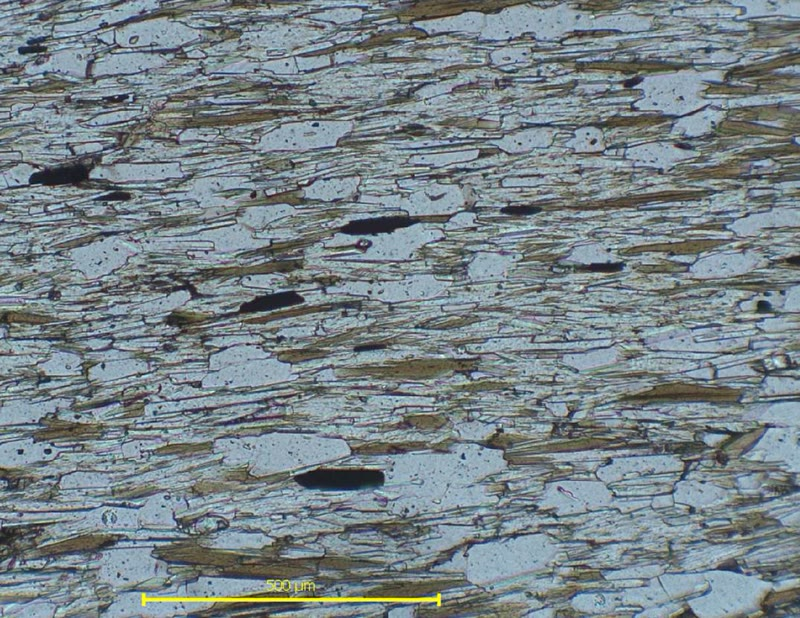
\includegraphics[height=4.3cm]{images/book2/g12-geoloshe-slaty-cleavage.jpg}\hspace{0.03\linewidth}%
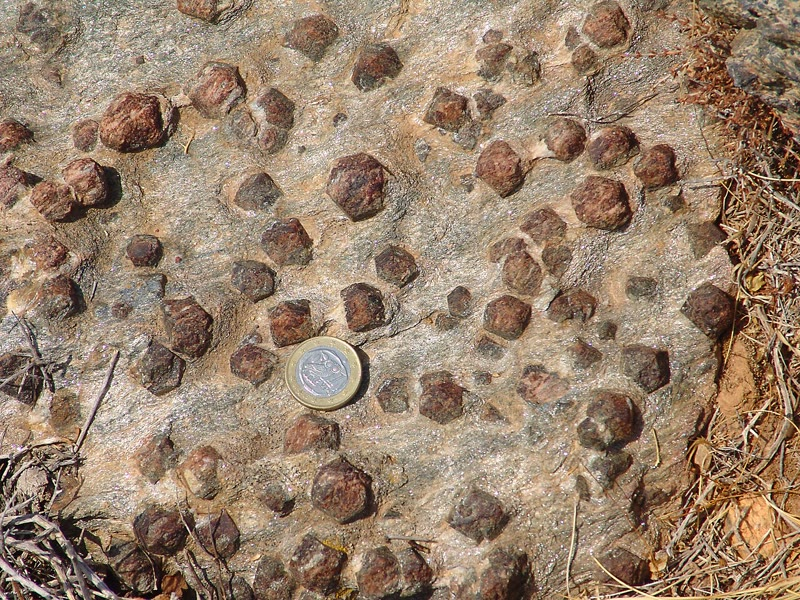
\includegraphics[height=4.3cm]{images/book2/g12-churchard-syros-garnet-schist.jpg}

\smallskip
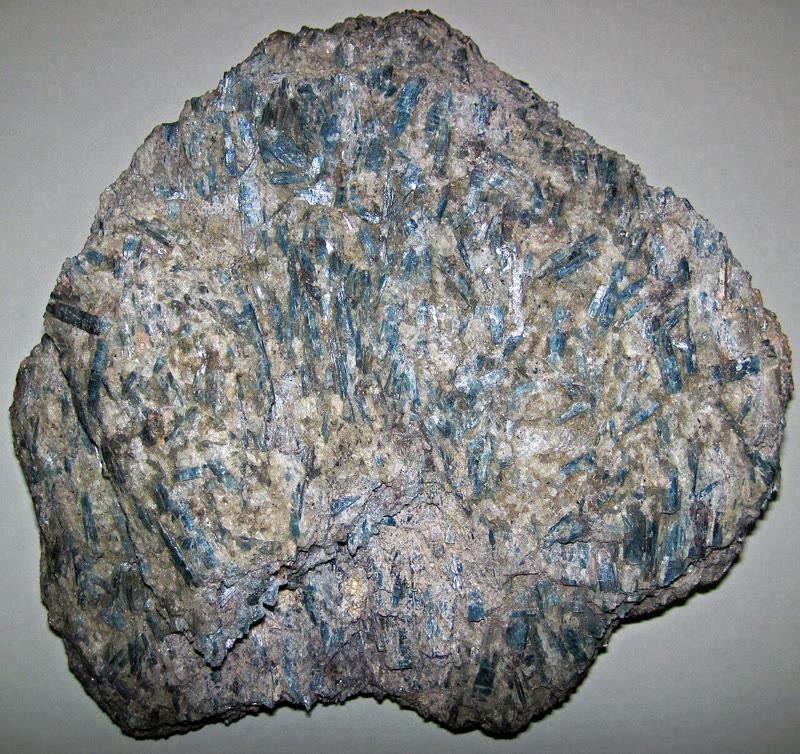
\includegraphics[height=4.3cm]{images/book2/g12-stjohn-kyanite-schist.jpg}\hspace{0.03\linewidth}%
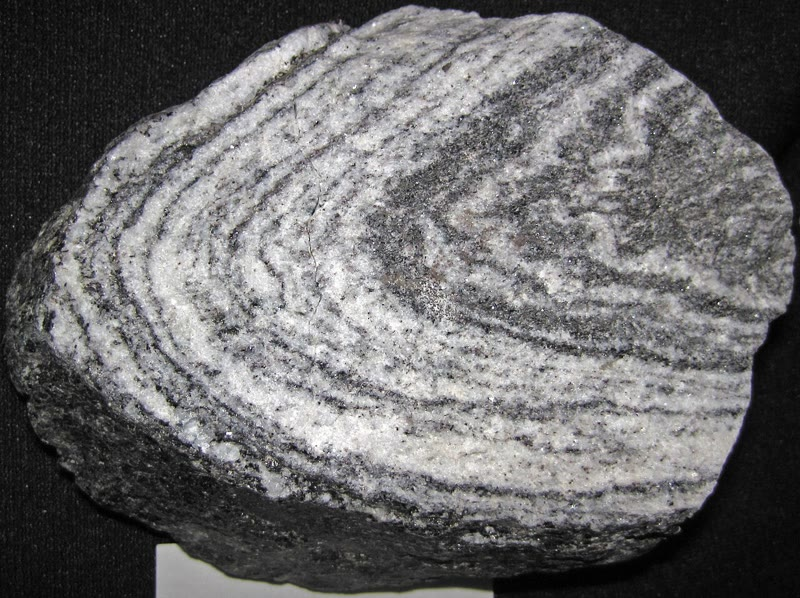
\includegraphics[height=4.3cm]{images/book2/g12-stjohn-gneiss.jpg}

{\small في الأعلى يمينًا: أردواز تحت المجهر (الشريط الأصفر طوله
\qty{500}{\micro\metre}): رقائق الميكا فيه كلها في اتجاه واحد.
في الأعلى يسارًا: شيست ميكا بالعقيق في جزيرة سيروس؛ وقطر القطعة النقدية
\qty{23}{mm}. في الأسفل يمينًا: شيست فيه نصال زرقاء من الكيانيت.
في الأسفل يسارًا: نيس بأشرطة من الكوارتز (فاتحة) ومن ميكا البيوتيت
(داكنة). الصور: جيولوشي (\babelsublr{CC0})، وغريم تشرتشارد (\babelsublr{CC~BY~2.0}) وجيمس
سانت~جون (\babelsublr{CC~BY~2.0}).}
\end{omfigure}
% ledger: photo:g12-slaty-cleavage, photo:g12-syros-schist, photo:g12-kyanite-schist, photo:g12-gneiss

على امتداد \omterm{def:g11:lithosphere-asthenosphere:geotherm}{منحنى حراري أرضي} نموذجي، يتكوّن الأردواز بين نحو 5 و\qty{10}{km}
تحت السطح، والفيليت بين 10 و15، والشيست بين 15 و20، والنيس بين
20 و\qty{25}{km}؛ وأعمق من ذلك، يبدأ الصخر بالانصهار في بعض المواضع.
\omterm{def:g12:metamorphic-rocks:foliation}{والتورق} يسجّل اتجاه العصر: فهو يتكوّن متعامدًا على
\omterm{def:g12:mountain-building:shortening}{التقصير} الذي يبني الجبال (\cref{ch:g12:mountain-building})، وقد
يظل التطبق الأصلي للوحل مرئيًا يقطعه بزاوية.
% ledger: earle:settings, earle:foliation

الصخور التي ليس فيها معادن مسطحة أو طويلة لا تُظهر تورقًا حتى حين
تُعصر. فالحجر الجيري يصير \textbf{رخامًا}، مكوّنًا من بلورات أكبر
من الكالسيت مُحيت فيها الأحافير؛ والحجر الرملي يصير
\textbf{كوارتزيتًا}، تداخلت حبيبات الكوارتز فيه بعضها في بعض؛
والوحل الذي يُسخَّن دون أن يُعصر يصير صخرًا صلبًا دقيق الحبيبات بلا
\omterm{def:g12:metamorphic-rocks:foliation}{تورق}، هو \textbf{الهورنفلس}.
% ledger: earle:foliation, earle:contact

\section{التحول التماسي والتحول الإقليمي}

\begin{definition}[التحول التماسي؛ التحول الإقليمي؛ هالة التحول]\label{def:g12:metamorphic-rocks:contact-regional}
\emph{التحول التماسي}\index{تحول تماسي} هو تحول
الصخور التي سخّنها جسم من الصهارة تداخل فيها؛ وهو محصور في
نطاق حول \omterm{def:g11:igneous-rocks:intrusion}{الجسم المتداخل}، هو \emph{هالة التحول}\index{هالة التحول}، التي
ترتفع فيها الدرجة نحو التماس. و\emph{التحول
الإقليمي}\index{تحول إقليمي} يصيب صخورًا دُفنت عميقًا في
مناطق واسعة، عادةً حيث تتقارب الصفائح؛ فتُعصر الصخور كما
تُسخَّن، وتكون متورقة في كل الحالات تقريبًا.
\end{definition}
% ledger: earle:contact, earle:regional, tulane:metamorphism

\subsection{حول جسم من الصهارة}

جسم من الصهارة عند نحو \qty{1000}{\celsius} يصعد في القشرة العليا
الباردة يسخّن الصخور المحيطة به. فقد تبلغ درجة حرارتها من 300 إلى أكثر
من \qty{800}{\celsius}، تحت الضغوط المنخفضة للأعماق الضحلة.
\omterm{def:g12:metamorphic-rocks:contact-regional}{وهالة التحول} ضيقة: بضعة سنتيمترات حول صفيحة رقيقة من الصهارة، وما يصل إلى
عدة عشرات من الأمتار حول جسم كبير. وصخورها تُسخَّن دون أن
تُعصر، فلا تكون متورقة: فالوحل يصير هورنفلسًا، والحجر الجيري
رخامًا، والحجر الرملي كوارتزيتًا. والجسم من الصهارة الذي يستقر عميقًا في صخور هي
ساخنة أصلًا لا يكاد يصنع هالة تحول.
% ledger: earle:contact, earle:settings (magma bodies around 1000 degC)

\begin{omfigure}
\begin{tikzpicture}[font=\scriptsize]
  \def\pluton{(3.0,0) .. controls (3.0,2.3) and (7.0,2.3) .. (7.0,0) -- cycle}
  \def\aureole{(2.45,0) .. controls (2.45,2.95) and (7.55,2.95) .. (7.55,0) -- cycle}
  \fill[lith sandstone] (0,0) rectangle (10,0.8);
  \fill[lith limestone] (0,0.8) rectangle (10,1.6);
  \fill[lith shale] (0,1.6) rectangle (10,3);
  \fill[omThm, opacity=0.30] \aureole;
  \draw[omThm, line width=0.6pt, dashed] (2.45,0) .. controls (2.45,2.95) and (7.55,2.95) .. (7.55,0);
  \fill[lith granite] \pluton;
  \draw[black!70, line width=0.6pt] (3.0,0) .. controls (3.0,2.3) and (7.0,2.3) .. (7.0,0);
  \draw[black!60] (0,0) rectangle (10,3);
  \node[fill=white, inner sep=1.5pt] at (5,0.45) {\foreignlanguage{arabic}{غرانيت، كان صهارة}};
  \draw[black!70] (6.0,1.95) -- (10.6,2.4) node[right] {\foreignlanguage{arabic}{هورنفلس، من الوحل}};
  \draw[black!70] (7.0,1.2) -- (10.6,1.2) node[right] {\foreignlanguage{arabic}{رخام، من الحجر الجيري}};
  \draw[black!70] (7.25,0.4) -- (10.6,0.4) node[right] {\foreignlanguage{arabic}{كوارتزيت، من الحجر الرملي}};
  \node[left] at (0,2.3) {سجيل};
  \node[left] at (0,1.2) {حجر جيري};
  \node[left] at (0,0.4) {حجر رملي};
  \draw[omThm] (4.2,2.05) -- (3.4,3.25) node[above, omThm] {هالة التحول};
\end{tikzpicture}

{\small \omterm{def:g12:metamorphic-rocks:contact-regional}{التحول التماسي}، في مقطع عرضي: جسم من الصهارة صعد
في صخور رسوبية متطبقة وسخّن حوله هالة تحول ضيقة (بالأحمر)،
تتبلور صخورها من جديد دون أن تُعصر. رسم تخطيطي: هالات \omterm{def:g12:metamorphic-rocks:metamorphism}{التحول} الحقيقية
يتراوح عرضها بين سنتيمترات وعشرات الأمتار.}
\end{omfigure}
% ledger: earle:contact

\subsection{تحت حزام جبلي}

يحتاج \omterm{def:g12:metamorphic-rocks:contact-regional}{التحول الإقليمي} إلى دفن حتى 10 أو \qty{20}{km}، فهو يصيب
آلاف الكيلومترات المربعة دفعة واحدة. وأرجح مكان له هو \omterm{def:g12:continental-crust:root}{جذر}
الحزام الجبلي، حيث يُسمّك الاصطدام القشرة ويدفع صخورها إلى الأسفل
(\cref{ch:g12:mountain-building}). ففي حزام قديم رُسمت خرائط
نطاقاته، سُخّنت صخور نطاق السيليمانيت فوق
\qty{700}{\celsius} ودُفنت على عمق 20 إلى \qty{25}{km}، في حين أن صخور
نطاق الكلوريت الخارجي ربما لم تُدفن قط أعمق من نحو \qty{5}{km}.
ثم بُليت الجبال التي فوقها على مدى عشرات ملايين السنين؛ وكلما
أُزيل الحمل، ارتفعت القشرة السميكة من جديد، فصارت النطاقات التي كانت عميقة
تقع الآن على السطح (\cref{ch:g12:destruction-of-mountains}).
% ledger: earle:regional

\subsection{ثلاثة منحنيات حرارية أرضية}

تُظهر \omterm{def:g12:metamorphic-rocks:polymorph}{متعددات الأشكال} بنظرة واحدة أن العمق نفسه لا يعني الصخر
نفسه في كل مكان: فذلك يتوقف على \omterm{def:g11:lithosphere-asthenosphere:geotherm}{المنحنى الحراري الأرضي}. ومخطط \omterm{def:g12:metamorphic-rocks:polymorph}{متعددات الأشكال}
يحمل ثلاثة منها.
% ledger: earle:settings

\begin{itemize}
  \item \omterm{def:g11:lithosphere-asthenosphere:geotherm}{منحنى حراري أرضي} \textbf{نموذجي}، نحو \qty{30}{\celsius} لكل
        كيلومتر: تبلغ درجة الحرارة نحو \qty{300}{\celsius} على عمق
        \qty{10}{km}. وهو يمر تحت النقطة الثلاثية، فيفسح الكيانيت
        المجال مباشرة للسيليمانيت، عند نحو \qty{574}{\celsius}
        و\qty{18.8}{km}.
  \item \omterm{def:g11:lithosphere-asthenosphere:geotherm}{منحنى حراري أرضي} في \textbf{منطقة بركانية}، من 40 إلى \qty{50}{\celsius} لكل
        كيلومتر، تزيد انحداره حرارة الصهارة الصاعدة: فالصخور تبلغ
        درجات حرارة عالية على أعماق ضحلة. وعند \qty{50}{\celsius} لكل
        كيلومتر، يظهر الأندالوسيت على عمق نحو \qty{6.6}{km} ثم يفسح المجال
        للسيليمانيت على عمق نحو \qty{10.9}{km}، عند \qty{553}{\celsius}.
  \item \omterm{def:g11:lithosphere-asthenosphere:geotherm}{المنحنى الحراري الأرضي} في \textbf{\omterm{def:g11:subduction-zones:subduction}{نطاق اندساس}}، دون
        \qty{10}{\celsius} لكل كيلومتر: \omterm{def:g11:ocean-ridges:oceanic-lithosphere}{فالقشرة المحيطية} المحمولة إلى الأسفل
        تبقى أبرد بعدة مئات من الدرجات من الوشاح المحيط بها. وعلى
        عمق \qty{36}{km} لا تزيد درجة حرارتها على نحو \qty{370}{\celsius}، في عمق
        حقل الكيانيت. وهذا هو المسار البارد العالي الضغط الذي يصير فيه البازلت
        شيستًا أزرق، ثم إكلوجيتًا، على عمق نحو \qty{35}{km}.
\end{itemize}
% values: cross_30_0 573.6 degC 18.79 km; cross_50_0 340.1 degC 6.60 km; cross_50_1 553.0 degC 10.86 km; sub10_T_at_1gpa 370.2 (al2sio5.py)
% ledger: earle:settings

وهكذا يحمل كل صخر متحول سجلًا \omterm{def:g11:lithosphere-asthenosphere:geotherm}{للمنحنى الحراري الأرضي} الذي
تكوّن تحته، وللبيئة الصفائحية التي وراءه: فالأندالوسيت والهورنفلس يشيران إلى
حرارة على أعماق ضحلة، حول أجسام من الصهارة؛ وشيست الكيانيت والسيليمانيت
ونيسهما إلى \omterm{def:g12:continental-crust:root}{الجذور العميقة} للأحزمة الجبلية؛ \omterm{def:g11:subduction-zones:eclogite}{والشيست الأزرق}
\omterm{def:g11:subduction-zones:eclogite}{والإكلوجيت} إلى نطاقات \omterm{def:g11:subduction-zones:subduction}{الاندساس}. ومعظم هذه الصخور ما كان ليُرى إلا
لأنها عادت إلى السطح دون أن تتحول عكسيًا. فهي إذ تصعد
وتبرد، تتباطأ تفاعلاتها، والماء الذي تحتاج إليه التفاعلات
العكسية كان قد أفلت في طريق النزول.
% ledger: earle:settings, earle:contact, tulane:metamorphism (retrograde metamorphism uncommon)

\section{تمارين}

\begin{exercise}[$\star$]\label{exo:g12:metamorphic-rocks:1}
اذكر المصطلح: (أ) معادن لها التركيب نفسه وبنى بلورية
مختلفة؛ (ب) الخط على الخريطة حيث يظهر \omterm{def:g12:metamorphic-rocks:index-mineral}{معدن دليلي} لأول مرة؛
(ج) نطاق الصخور المسخّنة حول جسم من الصهارة؛ (د) المستويات المتوازية
التي تصنعها المعادن المسطحة المصطفة؛ (ه) الضغط الناتج عن وزن
الصخور التي فوق.
\end{exercise}

\begin{exercise}[$\star$]\label{exo:g12:metamorphic-rocks:2}
سمّ الصخر المتحول الذي يصير إليه كل \omterm{def:g10:soil-formation:weathering-profile}{صخر أم}: (1) حجر جيري؛
(2) حجر رملي؛ (3) وحل، في درجة منخفضة تحت العصر؛ (4) وحل، في درجة
عالية؛ (5) وحل، سخّنه جسم من الصهارة دون أن يُعصر.
\end{exercise}

\begin{exercise}[$\star$]\label{exo:g12:metamorphic-rocks:3}
مع $\rho = \qty{2830}{kg/m^3}$ و$g = \qty{9.81}{m/s^2}$، احسب
\omterm{def:g12:metamorphic-rocks:lithostatic}{الضغط الصخري}، بوحدة \unit{GPa}، على عمق \qty{10}{km} وعلى عمق \qty{20}{km}.
\end{exercise}

\begin{exercise}[$\star$]\label{exo:g12:metamorphic-rocks:4}
على مخطط \omterm{def:g12:metamorphic-rocks:polymorph}{متعددات أشكال} \ce{Al2SiO5}، أي معدن يكون مستقرًا
(1) عند \qty{400}{\celsius} و\qty{0.6}{GPa}؛ (2) عند \qty{500}{\celsius}
و\qty{0.2}{GPa}؛ (3) عند \qty{750}{\celsius} و\qty{0.3}{GPa}؟
\end{exercise}

\begin{exercise}[$\star$]\label{exo:g12:metamorphic-rocks:5}
(1) رتّب بحسب ارتفاع الدرجة: الشيست، والأردواز، والنيس، والفيليت. (2) في
أيها يمكن رؤية الميكا بالعين المجردة؟ (3) أيها يُظهر
أشرطة فاتحة وداكنة؟
\end{exercise}

\begin{exercise}[$\star\star$]\label{exo:g12:metamorphic-rocks:6}
(1) احسب \omterm{def:g12:metamorphic-rocks:lithostatic}{الضغط الصخري} عند قاعدة قشرة سمكها \qty{35}{km}
($\rho = \qty{2830}{kg/m^3}$) وعبّر عنه بالضغط الجوي
($\qty{1}{atm} = \qty{101325}{Pa}$). (2) احسب الضغط على قاع
محيط عمقه \qty{4}{km}، بماء بحر كثافته
\qty{1025}{kg/m^3}. (3) كم مرة يفوق الأول الثاني؟
\end{exercise}

\begin{exercise}[$\star\star$]\label{exo:g12:metamorphic-rocks:7}
تقع النقطة الثلاثية للصيغة \ce{Al2SiO5} عند \qty{504}{\celsius}
و\qty{0.375}{GPa}. (1) على أي عمق يُبلغ ذلك الضغط ($\rho =
\qty{2830}{kg/m^3}$)؟ (2) أي \omterm{def:g11:lithosphere-asthenosphere:geotherm}{تدرج حراري أرضي}، يبدأ من
\qty{10}{\celsius} عند السطح، يمر بها تمامًا؟ (3) هل يُرجَّح أن يكون الصخر
الذي يحوي \omterm{def:g12:metamorphic-rocks:polymorph}{متعددات الأشكال} الثلاثة شائعًا؟
\end{exercise}

\begin{exercise}[$\star\star$]\label{exo:g12:metamorphic-rocks:8}
في صورة شيست العقيق من سيروس، يبلغ قطر أكبر حبات العقيق
نحو ثلث قطر القطعة النقدية، وهو \qty{23}{mm}. (1) قدّر
قطرها. (2) إذا كان قطر حبة العقيق يزداد بنحو \qty{1}{mm} في
مليون سنة، فكم استغرق نموها؟ (3) ماذا يخبرك ذلك
عن الزمن الذي يقضيه الصخر في العمق؟
\end{exercise}

\begin{exercise}[$\star\star$]\label{exo:g12:metamorphic-rocks:9}
يسير جيولوجي \qty{24}{km} نحو الغرب عبر حزام جبلي قديم،
ويسجّل صخورًا مصنوعة من الوحل. في البداية لا تحوي إلا الكلوريت والبيوتيت؛
ويظهر أول عقيق بعد \qty{6}{km}، وأول ستوروليت بعد
\qty{11}{km}، وأول كيانيت بعد \qty{15}{km}، وأول سيليمانيت
بعد \qty{20}{km}. (1) كم خط تساوي درجة عبر؟ سمّها بالترتيب.
(2) في أي اتجاه ترتفع الدرجة؟ (3) أين دُفنت الصخور
أعمق ما يكون، وما مقدار السخونة التي بلغتها هناك تقريبًا؟
\end{exercise}

\begin{exercise}[$\star\star$]\label{exo:g12:metamorphic-rocks:10}
يصعد جسم من الصهارة في طبقات من الوحل والحجر الجيري والحجر الرملي قرب
السطح. (1) سمّ الصخر الذي تصير إليه كل طبقة بجواره. (2) لماذا لا تكون هذه
الصخور متورقة؟ (3) يستقر جسم ثانٍ من الصهارة على عمق \qty{20}{km}، في
صخور قريبة أصلًا من \qty{500}{\celsius}. فلماذا لا يكاد يصنع هالة تحول؟
\end{exercise}

\begin{exercise}[$\star\star$]\label{exo:g12:metamorphic-rocks:11}
تُعصر طبقة من الوحل من الشرق والغرب خلال اصطدام،
وتنمو فيها الميكا وهي تُسخَّن. (1) كيف تستلقي الميكا: هل أوجهها المسطحة
مواجهة للشرق والغرب أم للشمال والجنوب؟ (2) هل \omterm{def:g12:metamorphic-rocks:foliation}{التورق} الذي يتكوّن
أفقي أم رأسي؟ (3) رخام وكوارتزيت عُصرا على النحو
نفسه لا يُظهران أي \omterm{def:g12:metamorphic-rocks:foliation}{تورق}. لماذا؟
\end{exercise}

\begin{exercise}[$\star\star\star$]\label{exo:g12:metamorphic-rocks:12}
بين 500 و\qty{700}{\celsius}، يقترب حد الكيانيت--السيليمانيت من
الخط المستقيم $P = 0.577 + 0.00209\,(T - 600)$، حيث $P$ بوحدة
\unit{GPa} و$T$ بوحدة \unit{\celsius}. \omterm{def:g11:lithosphere-asthenosphere:geotherm}{والمنحنى الحراري الأرضي} النموذجي هو $T = 10 + 30z$
($z$ بوحدة \unit{km})، و$P = 0.0278\,z$. (1) اكتب \omterm{def:g11:lithosphere-asthenosphere:geotherm}{المنحنى الحراري الأرضي} بحيث يكون $P$
دالة في $T$. (2) جد أين يعبر الحد: درجة الحرارة، والضغط،
والعمق. (3) على امتداد هذا المنحنى، أي \omterm{def:g12:metamorphic-rocks:polymorph}{متعدد أشكال} يكون مستقرًا فوق ذلك العمق
مباشرة، وأيها تحته مباشرة؟
\end{exercise}

\begin{exercise}[$\star\star\star$]\label{exo:g12:metamorphic-rocks:13}
(1) على امتداد \omterm{def:g11:lithosphere-asthenosphere:geotherm}{منحنى حراري أرضي} \omterm{def:g11:subduction-zones:subduction}{لنطاق اندساس} قدره \qty{10}{\celsius} لكل كيلومتر، يبدأ
من \qty{10}{\celsius}، ما درجة الحرارة على عمق \qty{35}{km}، حيث
يتكوّن \omterm{def:g11:subduction-zones:eclogite}{الإكلوجيت}؟ (2) وما هي على امتداد \omterm{def:g11:lithosphere-asthenosphere:geotherm}{منحنى حراري أرضي} نموذجي قدره
\qty{30}{\celsius} لكل كيلومتر؟ (3) ضع النقطتين على مخطط
\omterm{def:g12:metamorphic-rocks:polymorph}{متعددات الأشكال}: أي \omterm{def:g12:metamorphic-rocks:polymorph}{متعدد أشكال} يكون مستقرًا عند الأولى؟ (4) لماذا
يتكوّن \omterm{def:g11:subduction-zones:eclogite}{الشيست الأزرق} \omterm{def:g11:subduction-zones:eclogite}{والإكلوجيت} في نطاقات \omterm{def:g11:subduction-zones:subduction}{الاندساس} ولا يكادان يتكوّنان في أي مكان آخر؟
\end{exercise}

\begin{exercise}[$\star\star\star$]\label{exo:g12:metamorphic-rocks:14}
كثافات الكيانيت والسيليمانيت والأندالوسيت هي \num{3.61}
و\num{3.24} و\qty{3.15}{g/cm^3}. (1) احسب حجم \qty{1}{kg} من
كل منها، بوحدة \unit{cm^3}. (2) بأي نسبة مئوية يصغر حجم الكيانيت عن
الأندالوسيت المساوي له كتلةً؟ (3) فسّر، بفكرة أن الضغط العالي
يحابي الترتيب الذي يشغل أقل حيز، لماذا يشغل الكيانيت
حقل الضغط العالي في المخطط.
\end{exercise}

\begin{exercise}[$\star\star\star$]\label{exo:g12:metamorphic-rocks:15}
في حزام جبلي قديم، سُخّنت صخور نطاق السيليمانيت فوق
\qty{700}{\celsius} ودُفنت على عمق 20 إلى \qty{25}{km}. (1) احسب
الضغط على عمق 20 و\qty{25}{km}. (2) باستعمال خط
التمرين~12، جد أدنى درجة حرارة يكون عندها السيليمانيت مستقرًا عند
كل من هذين الضغطين. وهل تتفق \qty{700}{\celsius} مع السيليمانيت؟
(3) ما التدرجات الحرارية الأرضية، بدءًا من \qty{10}{\celsius} عند السطح، التي تقتضيها
\qty{700}{\celsius} على عمق 20 و\qty{25}{km}؟ (4) تكشفت الصخور
على السطح بعد نحو 40 مليون سنة. فبأي معدل متوسط أُزيلت
الصخور التي فوقها، بوحدة \unit{mm} في السنة؟
\end{exercise}

\begin{problem}[{مسألة نهاية الأسبوع --- تاريخ شيست كيانيت}]
\label{pb:g12:metamorphic-rocks:1}
% ledger: hm93:table11, cm95:crust, earle:controls, earle:settings, earle:regional, tulane:roots, tulane:metamorphism, iugs:barrow; Book 3: webmineral:polymorphs; Book 1: ussa76:sea-level
% values: pb_z_km 25.214, pb_grad 23.4, pb_kysil_P_at_600_gpa 0.577 (al2sio5.py); t_on_kysil(7.0) = 658.9
شيست جُمع من لبّ حزام جبلي قديم يحوي المسكوفيت
والبيوتيت والكوارتز وحبات عقيق يصل قطرها إلى \qty{8}{mm}، ونصالًا زرقاء من
الكيانيت؛ ولا يحوي سيليمانيت ولا أندالوسيت. وتحاليل المختبر
لعقيقه وبيوتيته تعطي الظروف التي تبلور فيها:
نحو \qty{600}{\celsius} و\qty{0.70}{GPa}. خذ $\rho =
\qty{2830}{kg/m^3}$، و$g = \qty{9.81}{m/s^2}$، و\qty{10}{\celsius} عند
السطح، وخط الكيانيت--السيليمانيت في التمرين~12، $P = 0.577 +
0.00209\,(T - 600)$.

\medskip
\noindent\textbf{الجزء الأول --- المعادن.}
\begin{enumerate}
  \item لماذا يُسمّى الصخر شيستًا؟ وأي معادنه تصنع
        \omterm{def:g12:metamorphic-rocks:foliation}{الشستوزية}؟
  \item الكيانيت والأندالوسيت والسيليمانيت تشترك في صيغة واحدة. اكتبها،
        واذكر المصطلح الدال على مثل هذه المعادن.
  \item كثافتا الكيانيت والأندالوسيت \num{3.61}
        و\qty{3.15}{g/cm^3}. فبأي نسبة مئوية يصغر حجم كيلوغرام من
        الكيانيت؟ وأيهما يحابيه الضغط؟
  \item في تتابع \omterm{def:g12:metamorphic-rocks:index-mineral}{المعادن الدليلية} لصخور الوحل، إلى أي نطاق
        ينتمي الصخر؟ وأي \omterm{def:g12:metamorphic-rocks:index-mineral}{خطوط تساوي الدرجة} عبر في طريق نزوله؟
  \item إذا كان قطر حبات العقيق يزداد بنحو \qty{1}{mm} في مليون
        سنة، فكم استغرق نمو أكبرها؟
\end{enumerate}

\medskip
\noindent\textbf{الجزء الثاني --- الضغط ودرجة الحرارة.}
\begin{enumerate}[resume]
  \item عند \qty{600}{\celsius}، فوق أي ضغط يكون الكيانيت مستقرًا بدلًا
        من السيليمانيت؟
  \item تحقق من أن النقطة (\qty{600}{\celsius}، \qty{0.70}{GPa}) تقع في
        حقل الكيانيت.
  \item غياب السيليمانيت يعطي أدنى ضغط عند
        \qty{600}{\celsius}. فما هو؟
  \item لو سُخّن الصخر أكثر عند \qty{0.70}{GPa}، فعند أي
        درجة حرارة كان كيانيته سيتحول إلى سيليمانيت؟
  \item عبّر عن \qty{0.70}{GPa} بالكيلوبار ($\qty{1}{kbar} =
        \qty{e8}{Pa}$) وبالضغط الجوي ($\qty{1}{atm} = \qty{101325}{Pa}$).
\end{enumerate}

\medskip
\noindent\textbf{الجزء الثالث --- عمق الدفن.}
\begin{enumerate}[resume]
  \item بكم ميغاباسكال يرتفع \omterm{def:g12:metamorphic-rocks:lithostatic}{الضغط الصخري} لكل
        كيلومتر؟
  \item على أي عمق كان الشيست حين تبلور؟
  \item ما أصغر عمق يسمح به غياب السيليمانيت
        (السؤال 8)؟
  \item أعد السؤال 12 بكثافة قدرها \qty{2700}{kg/m^3} للصخور
        التي فوقه. بأي نسبة مئوية يتغير العمق؟
  \item سمك \omterm{def:g12:continental-crust:continental-crust}{القشرة القارية} عادةً من 35 إلى \qty{40}{km}، ومن 50 إلى
        \qty{70}{km} تحت الأحزمة الجبلية. فهل تبلور الشيست في
        القشرة أم في الوشاح؟
\end{enumerate}

\medskip
\noindent\textbf{الجزء الرابع --- المنحنى الحراري الأرضي، وطريق العودة صعودًا.}
\begin{enumerate}[resume]
  \item ما متوسط \omterm{def:g11:lithosphere-asthenosphere:geotherm}{التدرج الحراري الأرضي} الذي تقتضيه \qty{600}{\celsius} عند ذلك
        العمق؟
  \item قارنه بتدرجات \omterm{def:g11:subduction-zones:subduction}{نطاق الاندساس} والقشرة
        النموذجية والمنطقة البركانية. فأي نوع من \omterm{def:g12:metamorphic-rocks:metamorphism}{التحول} صنع الصخر؟
  \item على امتداد \omterm{def:g11:lithosphere-asthenosphere:geotherm}{منحنى حراري أرضي} نموذجي قدره \qty{30}{\celsius} لكل كيلومتر، كم
        تكون درجة الحرارة عند عمق السؤال 12؟ وأي
        \omterm{def:g12:metamorphic-rocks:polymorph}{متعدد أشكال} يكون عندئذ مستقرًا عند \qty{0.70}{GPa}؟
  \item لإعادة الشيست إلى السطح، كان لا بد من إزالة كل الصخور التي فوقه.
        فبمعدل متوسط قدره \qty{0.5}{mm} في السنة، كم استغرق
        ذلك؟
  \item لماذا لم يتحول الكيانيت عائدًا إلى أندالوسيت في طريق الصعود؟
  \item لخّص: على أي عمق تبلور شيست الكيانيت هذا؟
\end{enumerate}
\end{problem}
